\section{Algoritmo propuesto}\label{sec:algorithm}

En este proyecto de fin de grado, se propone un algoritmo gen\'etico basado en \'arboles de decisi\'on cuyo objetivo es extraer informaci\'on de se\~nales de compra. Es decir, se pretende dise\~nar un \'arbol de decisi\'on que sirva como modelo para saber cu\'al es el momento id\'oneo para situar \'ordenes de compra y de venta en el mercado de valores y extraer beneficio.\\

\subsection{\'Arboles de decisi\'on}
El primer punto a tratar para dise\~nar el modelo, que se va  utilizar para extraer las se\~nales de compra y venta, es la estructura del \'arbol de decisi\'on. En primer lugar se expone la elecci\'on de las etiquetas. A continuaci\'on, se desarrollar\'a el contenido de los nodos, en otras palabras, las condiciones que dividen los caminos.\\

En cuanto a la clasificaci\'on de los d\'ias de bolsa, se propone un dise\~no con tres etiquetas:
\begin{itemize}
    \item Etiqueta \textit{Buy}. Un d\'ia clasificado con esta etiqueta, es un d\'ia bueno para comprar. Implica que el modelo env\'ia una se\~nal de compra y, consecuentemente, se debe colocar una orden de compra de acciones, tantas como nos sea posible con el capital disponible.
    \item Etiqueta \textit{Sell}. En el caso de que un d\'ia se clasifique con esta, signfica que es un buen d\'ia para vender. Implica que el modelo env\'ia una se\~nal de venta y, por tanto, se ha de colocar una orden de venta de todas las acciones que se tengan.
    \item Etiqueta \textit{Stop}. Es una etiqueta comod\'in que se usa cuando las condiciones de un camino no son concluyentes para decidir si hay que comprar o vender. En esta situaci\'on el modelo no env\'ia ninguna se\~nal.
\end{itemize}

Esta elecci\'on est\'a motivada por la necesidad de que el modelo sea capaz de transmitir se\~nales de compra y venta. La forma m\'as sencilla de conseguir estos env\'ios es utilizar dos etiquetas, una de compra y otra de venta. Pero, de ser as\'i, todos los caminos de condiciones llevar\'ian al modelo a una compra o a una venta. En ciertas ocasiones, el estado de la bolsa puede no ser determinante para decidir si es un momento de compra o de venta. Es entonces cuando aparece, de forma l\'ogica, la tercer etiqueta, ni es momento de comprar ni lo es de vender. \\

Una vez conocida la posible clasificaci\'on, se debe desarrollar cu\'ales van a ser las caracter\'isticas que van a definir la clase de un d\'ia. En otras palabras, es necesario conocer las condiciones que van a constituir los nodos. En el \'arbol se van a situar condiciones que dividen a los nodos en dos ramas, la que cumple la condici\'on y la que no. Por tanto, todos los nodos ser\'an de bifurcaci\'on binaria. Las reglas que se van a evaluar son de la forma: 
 \[indicador(parametros) <= pivote\].
 
 Donde $pivote$ es una un n\'umero real e $indicador$ es eso, un indicador de bolsa, con par\'ametros o no, seg\'un la naturaleza del indicador. Se ha usado la siguiente lista con indicadores cl\'asicos:
 
 \begin{itemize}
     \item MACD
     \item ATR
     \item ROC
     \item EMA
     \item SMA
     \item Momento
     \item HILL
     \item RSI
     \item OBV
     \item AD
     \item TRANGE
     \item BBANDS\_HIGH
     \item BBANDS\_LOW
 \end{itemize}
 
Se adjunta como anexo una breve explicaci\'on de cada uno de los indicadores utilizados.\\ 
 
 En el caso de algunos indicadores, como EMA (\textit{Exponential Moving Average}) o SMA (\textit{Simple Moving Average}), se hace necesaria una ligera modificaci\'on. Esto es debido a que al entrenar un \'arbol en un determinado periodo, en este aparecer\'an reglas como $EMA(10) <= 500$. La potencia del indicador $EMA$ se encuenta al comparar su valor con el valor actual de la acci\'on y observar si se ha producido una bajada o subida importante respecto a los \'ultimos d\'ias.  

 
 		\begin{figure}[H]
    		\centering
    		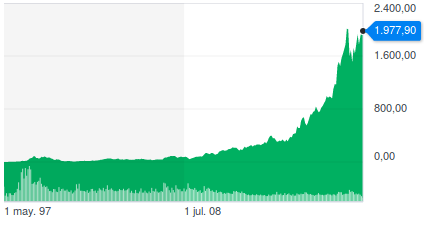
\includegraphics[scale=0.7]{imagenes/amazon.png}
    	    \caption[Valor de las acciones de Amazon en un periodo concreto]{Valor de las acciones de Amazon.\\ Fuente: \url{https://finance.yahoo.com} [\'Ultima consulta 19 de Julio de 2019]}
    		\label{fig:amazon}
	   \end{figure}
	   
En ciertos casos, por ejemplo en tendencias laterales, podr\'ia tener sentido usar esta condici\'on. Si el valor de la acci\'on lleva unos d\'ias demasiado alto o demasiado bajo puede signficar un cambio de tendencia.\\

Pero, en otros casos, resulta fatal. Imaginemos que nuestro modelo aprende en un periodo de entrenamiento en que una condici\'on con $EMA$ es muy significante. Al pasar al periodo de prueba, esta condici\'on puede ser absurda, como en el caso que se ve en la figura \ref{fig:amazon} de Amazon. El valor es solo creciente, no tiene sentido poner un pivote fijo.\\

En su lugar, se propone modificar este indicador restando o dividiendo a su valor el precio actual de la acci\'on para, de alguna forma, escalar el indicador y hacerlo intemporal. En el caso de la divisi\'on, se obtiene la proporci\'on entre el valor actual y un valor representante de los \'ultimos d\'ias. Por su parte, la resta es un poco menos aconsejable, ya que hay una gran diferencia entre que una acci\'on a 2 euros suba 10, y que una acci\'on de 500 euros suba 10. Ambos casos son positivos, pero el primero es mucho m\'as significativo. \\


\subsection{Estructura gen\'etica}
Para construir el \'arbol modelo, se utilizar\'a un patr\'on gen\'etico como el explicado en el apartado \ref{sec:genetico}, en el que, oportunamente, se hizo una explicaci\'on gen\'erica de un algoritmo gen\'etico. A continuaci\'on se procede a replicar esa construcci\'on adapt\'andola a nuestra poblaci\'on, los \'arboles de decisi\'on.\\

En primer lugar, se crea una generaci\'on y, mediante una simulaci\'on de inversi\'on en un periodo de prueba, se puntuan los \'arboles. A continuaci\'on se realiza un proceso de selecci\'on y de cruce de los \'arboles. Y por \'ultimo, se sortea una serie de mutaciones. Una vez terminado el procedimiento, vuelve a comenzar el proceso de simulaci\'on para encontrar la pr\'oxima generaci\'on.\\

A continuaci\'on se va a profundizar en cada uno de los pasos seguidos en este procedimiento.\\

\subsubsection{Primera generaci\'on}
La primera generaci\'on en los algoritmos gen\'eticos suele ser aleatoria y la l\'ogica de los siguientes pasos va perfilando y mejorando la poblaci\'on a largo plazo.\\

Puesto que nuestra simulaci\'on se prev\'e costosa, se va a proceder a realizar un ligero calentamiento de la poblaci\'on para que se reduzcan las iteraciones necesarias hasta la obtenci\'on de una poblaci\'on buena. Con el fin calentar los \'arboles en la primera poblaci\'on, se propone usar una construcci\'on con algunos elementos aleatorios y otros heur\'isticos.\\

En primer lugar, para cada \'arbol se toman indicadores de forma aleatoria que conforman los nodos. Cada vez que se a\~nade un nuevo nodo con su indicador, el pivote que divide los datos se toma a partir de los mejores resultados de una funci\'on de entrop\'ia. La funci\'on de entrop\'ia se aplica sobre los datos del periodo de prueba. A continuaci\'on se explicar\'a detalladamente cada paso. \\

\paragraph{Etiquetado de datos de prueba}
El mismo periodo que se va a usar para entrenar el algoritmo gen\'etico va a ser utilizado para generar esta primera poblaci\'on. As\'i pues, se toman estos datos y se etiquetan siguiendo estas consideraciones:

    Nombremos m\'axima subida, y lo notamos como $M$, a la siguiente expresi\'on:\\
    \begin{align*}
    \begin{split}
        M = max\{cierre_{i} - cierre_{j} \:|\: \forall z\: con \:i < z\leq j\: cierre_{z-1} - cierre_{z} \geq 0 \}
    \end{split}
    \end{align*}
    
    De forma an\'aloga, se obtiene la m\'axima bajada, notada como m:
    \begin{align*}
    \begin{split}
        m = max\{cierre_{i} - cierre_{j} \:|\: \forall z\: con \:i < z\leq j\:s cierre_{z-1} - cierre_{z} \leq 0 \}
    \end{split}
    \end{align*}

    Seguidamente, se definen dos tipos de tendencias.\\
    
    Una consecuci\'on de d\'ias tiene tendencia positiva siempre que en mitad no se halle una bajada del precio superior a la sexta parte de m.\\
    
    De forma an\'aloga, una consecuci\'on de d\'ias se dice con tendencia negativa si en mitad se halla una subida superior a la sexta parte de M.\\
    
    Es decir,
    
    \begin{align*}
    \begin{split}
        \{i,i+1,...,j\}\: \text{tiene tendencia positiva} \Longleftrightarrow{}\\
        \forall z,k\: con \:i < k < z\leq j\hspace{0.5cm} cierre_{z} - cierre_{k} \geq m/6
    \end{split}
    \end{align*}
    
    \begin{align*}
    \begin{split}
        \{i,i+1,...,j\}\: \text{tiene tendencia negativa} \Longleftrightarrow{}\\
        \forall z,k\: con \:i < k < z\leq j\hspace{0.5cm} cierre_{z} - cierre_{k} \leq M/6
    \end{split}
    \end{align*}

    En \'ultima instancia, se marcan los datos con cuatro etiquetas:
    \begin{itemize}
        \item \textbf{-2} para el \'ultimo d\'ia de cada tendencia negativa.
        \item \textbf{-1} para el resto de d\'ias de las tendencias negativas.
        \item \textbf{2} para el \'ultimo d\'ia de cada tendencia positiva.
        \item \textbf{1} para el resto de d\'ias de las tendencias positivas.
    \end{itemize}
    
    Estas etiquetas son un intento de marcar las diferencias de d\'ias buenos para comprar y d\'ias buenos para vender. \\
    
    En consecuencia, al sumar las etiquetas de un grupo de d\'ias, cuanto m\'as negativo sea el resultado, m\'as influencia tienen los m\'inimos de las tendencias negativas y, por tanto, los d\'ias est\'an orientados a comprar.\\
    
    En el caso contrario, una suma positiva implica una buena fecha para vender.\\
    
    En la figura \ref{fig:tagging} se puede observar un ejemplo simple de etiquetado de un periodo. En ella se ven los tramos clasificados como crecientes en azul y los decrecientes en rojo. Hay que destacar que la transici\'on de $D$ a $E$ es positiva, pero est\'a en mitad de un tramo decreciente y la diferencia no supera la sexta parte de la subida permitida por lo que, seg\'un lo anteriormente expuesto, se marca tambi\'en como decreciente.\\
    
     	\begin{figure}[H]
    		\centering\leftskip=-20px
    		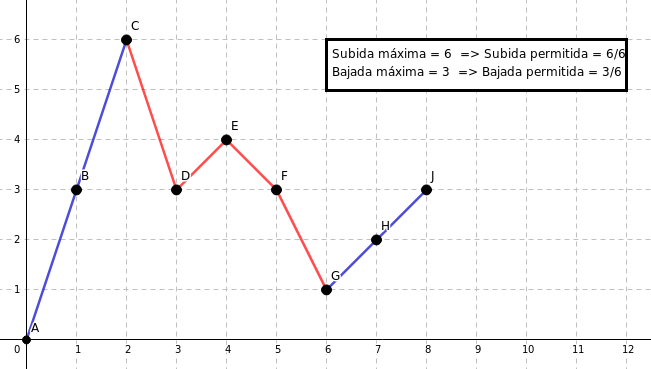
\includegraphics[scale=0.65]{imagenes/tagging.png}
    	    \caption[Ejemplo de etiquetado de un periodo]{Ejemplo de etiquetado de un periodo.\\ Fuente: elaboraci\'on propia}
    		\label{fig:tagging}
	   \end{figure}
    
\paragraph{Selecci\'on de pivotes}
Una vez se ha seleccionado un indicador para el nodo de un \'arbol de la primera generaci\'on, de forma aleatoria, el pivote se selecciona de forma heur\'istica. Hay que destacar que el pivote seleccionado no es el mejor de todos los posibles, simplemente se considera una elecci\'on para rectificar la aleatoridad de la selecci\'on de indicadores.\\

El pivote final elegido es un valor de una rejilla conformada por diez valores equidistantes situados entre el m\'aximo y el m\'inimo valor del par\'ametro de los datos que cumplen las condiciones para llegar al nodo. \\

Puesto que tenemos cuatro etiquetas, en primera instancia se deber\'ia usar una funci\'on de entrop\'ia de cuatro clases. Pero las etiquetas 2 y -2 son poco frecuentes. Adem\'as, debido a que nuestros nodos dividen los datos en dos ramas, no parece oportuno usar una entrop\'ia de cuatro clases. En su lugar proponemos hacer dos clases, una para las etiquetas negativas (-1 y -2), y otra para las positivas (1 y 2).\\

La funci\'on de entrop\'ia de dos clases es, por tanto:\\

$entropy(x) = x*log_{2}(x) + (1-x)log_{2}(1-x) \quad x\in(0,1)$\\

Donde $x$ es la proporci\'on de una de las clases. De este modo, en caso de que la proporci\'on de una clase sea 1, se obtiene la informaci\'on perfecta (la rama solo tiene datos de una clase), pero entonces, la funci\'on entrop\'ia no puede calcularse. Hay que tener en cuenta este caso especial  y evitar realizar el c\'alculo de la funci\'on.\\

Para calcular el mejor pivote de un nodo, se eval\'uan las entrop\'ias de las dos ramas que forma y se hace la suma proporcional al n\'umero de individuos. El pivote cuya funci\'on de entrop\'ia sea mayor es seleccionado como mejor pivote de la rejilla.\\

\paragraph{Selecci\'on de las hojas}
Cuando los datos que cumplen las condiciones de una rama son pocos o la rama ya tiene demasiada profundidad en este calentamiento de la primera generaci\'on, es necesario dar por terminada la rama y culminar la construcci\'on con una hoja.\\

Las hojas son, simplemente, una de las tres se\~nales posibles que permite el modelo propuesto: comprar, vender o no hacer nada.\\

Para escribir la decisi\'on que se debe tomar en esa hoja se va a usar una vez m\'as la etiqueta puesta en los datos de prueba. Notando $x_{tag=a}$ al n\'umero de instancias de los datos que cumplen el camino de condiciones y cuya etiqueta es $a$, definimos la variable que va a determinar la acci\'on de la hoja como:\\

$\alpha = \frac{x_{tag>0}\; -\; x_{tag<0} \; + \; x_{tag=2} \; -\; x_{tag=-2}}{x_{tag>0}\; + \; x_{tag<0}} $\\


Es importante destacar que, para cada hoja, los datos a tratar son aquellos que cumplen las condiciones del camino de nodos hasta la hoja. De este modo, por tanteo se llega a la siguiente adjudicaci\'on de la se\~nal de la hoja:\\

\[   
\text{se\~nal} = 
     \begin{cases}
       \text{Comprar} &\quad\text{si}\quad \alpha < -2\\
       \text{Stop} &\quad\text{si}\quad -2 \leq \alpha \leq 2\\
       \text{Vender} &\quad\text{si}\quad 2 < \alpha\\ 
     \end{cases}
\]

De forma coherente a la se\~nal que se quiere enviar, se colocan las etiquetas.\\

\subsubsection{Cruce}
En cada iteraci\'on del algoritmo se eval\'ua la poblaci\'on con \textit{backtrader} para simular los beneficios que cada individuo tendr\'ia en el periodo de prueba. Una vez extra\'idos los beneficios, se procede a generar la nueva poblaci\'on mediante un cruce que promocione a los \'arboles que mejores resultados han dado.\\

De entre las distintas formas que hay para seleccionar los individuos que se van a reproducir, se escoge la selecci\'on proporcional. M\'as tarde, se explicar\'a el cruce natural de dos \'arboles de decisi\'on\footnote{V\'ease la secci\'on \ref{sec:cruce}}.\\

Este cruce natural entre \'arboles tiene una peque\~na desventaja, y es que puede generar peores poblaciones que las progenitoras. Se hace pr\'acticamente indispensable, entonces, que activemos los m\'etodos elitistas y eliminatorios. Los mejores \'arboles pasar\'an dos veces a la siguiente generaci\'on, una vez mutados y otra vez sin modificar. Por su parte, los peores se descartar\'an por completo tanto del cruce como de la mutaci\'on.\\

\paragraph{Probabilidades de reproducci\'on}
En primer lugar, hay que calcular la probabilidad de cruce de cada individuo. Para ello se hace una normalizaci\'on especial de los beneficios.\\

Restando el beneficio del peor \'arbol a las puntuaciones de todos, se consigue que estas sean siempre mayores o iguales que 0.\\

A continuaci\'on, con el fin de potenciar las estrategias de compra y venta m\'ultiple, m\'as ventajosas que la estrategia de \textit{buy\&hold}\footnote{La estrategia \textit{buy\&hold} es una estrategia cl\'asica que se basa en la compra inicial de todas las acciones posibles y la venta final de las mismas. Esta estrategia recibe su nombre por la l\'ogica que sigue: comprar y mantener.}, se van a modificar ligeramente las ganacias. Por cada venta que produzca un \'arbol, se suma una cantidad fija de euros a sus beneficios. No obstante, para ciertos valores demasiado altos de esta cantidad con los que se supere las comisiones, las compras y ventas se realizar\'an de forma compulsiva. Es importante, por consiguiente, ajustar bien este valor para evitar este resultado.\\

En el \'ultimo paso de la normalizacion, se dividen todas las puntuaciones entre la suma de las puntuaciones. Esto produce que la suma de las mismas sea 1 y, adem\'as, cada valoraci\'on es proporcional a la cantidad de beneficios que reporta, a excepci\'on de la cantidad a\~nadida en favor de las transacciones r\'apidas.\\

Por \'ultimo, tomando $x \sim U[0,1]$ y notando $p_i$ como la puntuaci\'on normalizada del \'arbol i-\'esimo, se pueden sortear los individuos que se reproducen de forma proporcional a su beneficio de la siguiente forma:\\

\[   
seleccionado = 
     \begin{cases}
       \text{\'arbol 1} &\quad\text{si}\quad 0 \leq x < p_1\\
       \text{\'arbol 2} &\quad\text{si}\quad p_1 \leq x < p_1 + p_2\\
       \text{...} \\
       \text{\'arbol n} &\quad\text{si}\quad \sum\limits_{i=1}^{n-1} p_i \leq x \leq \sum\limits_{i=1}^{n} p_i = 1\\ 
     \end{cases}
\]

Son necesarios dos \'arboles para realizar un cruce, del que, a su vez, resultan otros dos \'arboles. Se tienen que ejecutar tantas selecciones como sean necesarias para que la siguiente generaci\'on mantenga el n\'umero de individuos.\\

Una anotaci\'on final es necesaria. En el caso especial de que todos los \'arboles tengan los mismos beneficios, este procedimiento llevar\'ia a dividir por 0. Para evitar esto, de forma natural se divide el intervalo [0,1] en tantos intervalos de igual dimensi\'on como \'arboles haya y continuamos con el caso general. A cada \'arbol se le asigna un intervalo, esta vez, al ser todos iguales, no importa cu\'al y la funci\'on de selecci\'on podr\'ia ser la siguiente:\\

\[   
seleccionado = 
\begin{cases}
\text{\'arbol 1} &\quad\text{si}\quad 0 \leq x < \frac{1}{n}\\
\text{\'arbol 2} &\quad\text{si}\quad \frac{1}{n} \leq x < \frac{2}{n}\\
\text{...} \\
\text{\'arbol n} &\quad\text{si}\quad \frac{n-1}{n} \leq x \leq 1\\ 
\end{cases}
\]



\paragraph{Cruce natural entre dos \'arboles}\label{sec:cruce}
El cruce entre individuos de la poblaci\'on es el mecanismo central de los algoritmos gen\'eticos. En nuestra propuesta, al tener una poblaci\'on de \'arboles, se va a usar el cruce natural entre estos. \\

Como ya se ha introducido en el punto anterior, con este cruce propuesto no se asegura que los \'arboles de una generaci\'on sean mejores que los progenitores. No obstante, entendemos que es una buena forma de agrupar condiciones y de crear asociaciones diferentes de estas. En consecuencia, esto permite explorar el espacio de b\'usqueda de forma que una generaci\'on contenga modelos parecidos para la predicci\'on en bolsa.\\


El cruce parte de dos \'arboles, llamados padres o progenitores. En cada \'arbol progenitor se marca, con un patr\'on aleatorio, un nodo. Es indispensable que dicho nodo no sea una hoja, aunque s\'i podr\'ia ser la ra\'iz. \\

     	\begin{figure}[H]
    		\centering
    		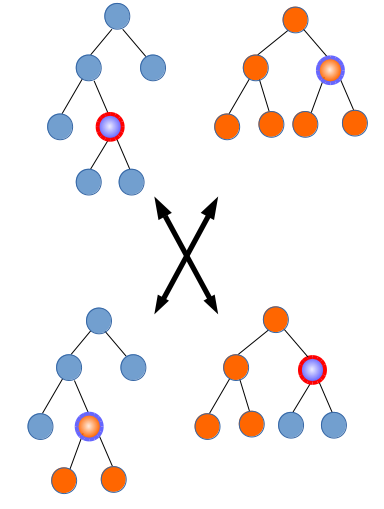
\includegraphics[scale=0.6]{imagenes/crossover.png}
    	    \caption[Ejemplo de cruce entre dos \'arboles]{Ejemplo de cruce entre dos \'arboles.\\ Fuente: elaboraci\'on propia}
    		\label{fig:crossover}
	   \end{figure}

Para construir a los hijos, se intercambian sendos nodos seleccionados y, con ellos, todos los nodos que penden de \'el. En la figura \ref{fig:crossover} puede verse una descripci\'on gr\'afica del cruce.\\

Este cruce puede producir varias anomal\'ias al iterar. Una de ellas es la generaci\'on de \'arboles con una profundidad extrema. Es decir, la poblaci\'on tiene una cierta probabilidad de converger a \'arboles con demasiados nodos o, en su defecto, con insuficientes nodos.\\


     	\begin{figure}[H]
     		\centering
     		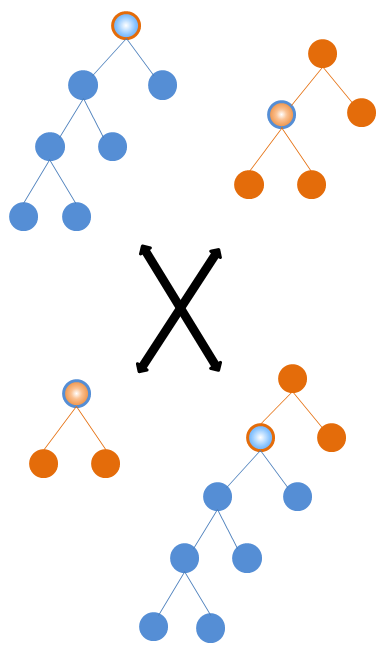
\includegraphics[scale=0.4]{imagenes/small_crossover.png}
     		\caption[Ejemplo de generaci\'on de un \'arbol peque\~no]{Ejemplo de generaci\'on de un \'arbol peque\~no y otro grande.\\ Fuente: elaboraci\'on propia}
     		\label{fig:small_crossover}
     	\end{figure}


Por lo general, un exceso de nodos, que puede entenderse como un exceso de condiciones, va a producir modelos muy espec\'ificos. Los \'arboles demasiado espec\'ificos suelen aprender muy bien la casu\'istica de los dos datos de prueba. Sin embargo, fallan al intentar extenderse al periodo de prueba. Esto es lo que en el \'ambito de la ciencia de datos se denomina sobreaprendizaje.\\

En contraposici\'on, un \'arbol con pocas condiciones o nodos, va a tender a generalizar demasiado las situaciones y, a menudo, no son capaces si quiera de obtener un bueno modelo para los datos de entrenamiento.\\

Para solventar estos dos problemas se actuar\'a de la siguiente forma:\\

\begin{itemize}
    \item La selecci\'on de nodo a intercambiar en el cruce no se hace de forma uniforme. Empezando desde el nodo ra\'iz y con igual probabilidad, se sortea si el nodo elegido para intercambio presenta una de estas tres posibilidades: el actual, est\'a en la rama izquierda o est\'a en la rama derecha. Por consiguiente, es m\'as probable que se tome un nodo cercano a la ra\'iz para hacer el cambio. N\'otese que no es posible intercambiar una hoja, luego si en este procedimiento se llega a una hoja, el nodo a intercambiar es el inmediatamente superior.\\
    
    En un intento de justificar la anulaci\'on de las hojas como punto de mutaci\'on se pide reflexionar sobre el siguiente caso extremo. Para generar dos nuevos \'arboles, los progenitores han marcado como punto de corte una hoja, el primer progenitor, y la ra\'iz, el segundo. Por tanto, al generar a los nuevos hijos, el primer \'arbol ser\'ia el primer progenitor al completo al que se le ha a\~nadido el segundo en una hoja. El segundo hijo, por su parte, remplazar\'ia todo el segundo \'arbol progenitor por una hoja del primero. Esto es, el segundo hijo no tienes nodos y, se entiende que en este caso especial, clasifica todos los d\'ias con la misma etiqueta, la que aparece en su \'unica hoja. \\
    
    Esta forma condicionada de seleccionar los nodos tiene como objetivo evitar la formaci\'on de \'arboles muy peque\~nos. Ya que, para que una rama grande se sustituya por una rama peque\~na, es necesario que la selecci\'on de nodo baje mucho en la jerarqu\'ia. Pero la probabilidad de que la selecci\'on baje mucho es una probabilidad condicionada m\'ultiples veces.\\
    
    \item Para eliminar los \'arboles demasiado grandes, simplemente se propone desarrollar un m\'etodo que cuente los nodos de un \'arbol y, en cada generaci\'on, se eliminen los que superen una cierta cantidad. A pesar de que el m\'etodo anterior parece efectivo para controlar los \'arboles peque\~nos, tambi\'en se ha a\~nadido el caso contrario: si hay pocos nodos en un \'arbol, \'este se elimina. \\
    
    De forma inicial, hemos acotado los nodos de un \'arbol entre 15 y 45. No obstante estas cifras son orientantivas, tras ver algunos resultados podr\'ia ser conveniente cambiarlas.\\
    
    Para mantener constante la cantidad de inviduos por poblaci\'on, se tienen que cruzar tantos \'arboles como la mitad de eliminaciones se hallan producido.\\
\end{itemize}

\subsubsection{Mutaciones}
Tal y como se han presentado el cruce y la primera generaci\'on, hay varios factores de la poblaci\'on que no es posible alterar, estos son:\\

\begin{itemize}
    \item \textbf{Los par\'ametros de los indicadores.} Algunos indicadores, como el EMA (Exponential Moving Average), depende de uno o varios par\'ametros. En primera instancia se han impuesto unos valores, con cierta variabilidad, para ellos. El cruce permite cambiar los nodos de posici\'on y, a la larga, cambiar las combinaciones de indicadores pero, en ning\'un caso, se produce un cambio en los par\'ametros de los indicadores. Los valores impuestos para estos en un inicio no tienen por qu\'e ser \'optimos. Adem\'as, la idoneidad de un valor depende, en cierta medida, del conjunto de indicadores que precedan a la condici\'on. Se crea, entonces, la necesidad de establecer un mecanismo para cambiarlos.
    \item \textbf{La combinaci\'on entre el \'ultimo nodo y las etiquetas.} El cruce propuesto no permite mover las hojas, salvo en el caso de que lo que se mueva sea un nodo superior. Esto hace que las se\~nales vayan asociadas a unos indicadores elegidos en la primera iteraci\'on de forma aleatoria lo que, a poco que se piense, parece una dura restricci\'on. Es necesario crear un m\'etodo que cambie las etiquetas. 
    \item \textbf{Los pivotes de cada nodo.} A partir de la funci\'on de entrop\'ia y los datos de entrenamiento se eligen los primeros pivotes de la primera generaci\'on. Pero una vez que el nodo cambia de posici\'on a causa del cruce, el pivote no tiene por qu\'e estar bien elegido. Es necesario entonces un proceso para cambiar los pivotes.
\end{itemize}

 El mecanismo que desarrollaremos en los sucesivos ep\'igrafes, con el que podemos alterar todos estos factores est\'aticos, es la mutaci\'on.\\
 
 Las mutaciones suceden con cierta probabilidad sobre distintos lugares de los individuos. Seg\'un la naturaleza de estos, se pueden plantear distintos m\'etodos de mutaci\'on.\\
 
 En nuestro caso, se ir\'a recorriendo el \'arbol nodo por nodo desde la ra\'iz hasta las hojas. En cada nodo se toma un entero aleatorio en un rango dado. Seg\'un el valor extra\'ido, se ejecuta una mutaci\'on de par\'ametros, de pivotes, de indicadores de hojas (en caso de que el nodo fuese una hoja) o ninguna. A continuaci\'on se desarrolla cada mutaci\'on.\\

\paragraph{Mutaciones en indicadores}
El cruce permite cambiar la composici\'on de condiciones que conforman el modelo. No obstante, es un cambio muy general. En ocasiones, cambiando un \'unico indicador de un nodo en mitad de una rama se produce un cambio muy positivo.\\

Ya sea con el objetivo de provocar estos cambios o simplemente para explorar m\'as \'arboles en el espacio de b\'usqueda similares a la generaci\'on anterior, se propone que, de forma aleatoria, se tome una nueva funci\'on indicadora que suplante a la anterior. \\

En consecuencia con este cambio, mantener el pivote que se situaba en el mismo nodo carece de sentido, pues cada indicador tiene su imagen en una horquilla distinta de valores. Se hace obligatorio, por tanto, recalcular el pivote del nodo.\\  

\paragraph{Mutaciones en los pivotes}

Todos los indicadores utilizados tienen su imagen contenida en $\mathbb{R}$, luego los pivotes que condicionan el nodo tambi\'en. Existen varias formas de mutar un valor real. Aqu\'i se propone introducir un ruido basado en la normal.\\

En cada mutaci\'on de pivote, el nuevo pivote es un valor extra\'ido de una distribuci\'on normal $N(pivote, |pivote/4|)$, es decir, se saca de una normal centrada en el antiguo valor y con varianza la cuarta parte del antiguo valor.\\

\paragraph{Mutaciones en par\'ametros de indicadores}
La mutaci\'on de par\'ametros es espec\'ifica, seg\'un el indicador al que pertenezca.\\

Los par\'ametros que se mueven en $\mathbb{R}$ pueden calcularse, igual que la mutaci\'on de pivotes, a partir de una distribuci\'on normal. En el caso de que el par\'ametro se mueva en $\mathbb{R}_0^+$, como en el caso de las \textit{Bollinger Bands}, se debe rectificar con un valor absoluto.\\

En cuanto a los par\'ametros que se mueven en $\mathbb{N}$ o subconjuntos del mismo, optamos por hacer una mutaci\'on discreta sumando o restando 2. \\

\paragraph{Mutaciones en las hojas}
Las mutaciones en una hoja son bastante sencillas. Una hoja puede tener los valores \textit{'Compra'}, \textit{'Vende'} o \textit{'Stop'}. Basta con tomar una nueva etiqueta de forma aleatoria.\\


